\documentclass[12pt,a4paper]{article}
\usepackage[a4paper,top=12mm,bottom=14mm,left=15mm,right=15mm]{geometry}
\usepackage[T1]{fontenc}
\usepackage{amsmath}
\usepackage{amssymb}
\usepackage{enumitem}
\usepackage{multicol}
\usepackage{xcolor}
\usepackage{tikz}
\usepackage[most]{tcolorbox}
\usetikzlibrary{arrows.meta}

% ================================================================
% The Chinese multiplication method.
%
% A Key Stage 3 arithmetic sheet, designed to be worked through
% alone: the method is introduced by a worked example, then
% practised in three stages of decreasing support -- a grid that is
% already filled in, so that only the diagonal addition is left; a
% grid that is drawn but empty; and finally no grid at all. The
% decimal point runs through the whole sheet, first with both
% numbers written as decimals and then with one of them whole.
% Answers are on the last page so that pupils can check each part
% before going on.
%
% The sheet is written on, so every question is followed by a
% working area. The \newpage commands in the body are placed so
% that no question is split across the fold.
% ================================================================

\pagestyle{empty}
\linespread{1.15}\selectfont
\setlength{\parskip}{5pt}
\setlist[enumerate,1]{label=\textbf{Q\arabic*.}, leftmargin=*, itemsep=10pt, topsep=6pt, parsep=4pt}
\setlist[enumerate,2]{label=(\alph*), leftmargin=*, itemsep=8pt, topsep=5pt, parsep=3pt}
\setlength{\multicolsep}{4pt}
\setlength{\parindent}{0pt}

\newcommand{\ansline}[1][2.2cm]{\underline{\hspace{#1}}}

% A worked example: the method shown in full before it is practised.
\newtcolorbox{wex}[1]{colback=blue!4,colframe=blue!45!black,boxrule=0.6pt,
  left=6pt,right=6pt,top=4pt,bottom=5pt,
  title={\bfseries\small Worked example: #1},fonttitle=\small,
  toptitle=1pt,bottomtitle=1pt}

% The idea a section is built on, stated once and boxed.
\newtcolorbox{keyidea}{colback=orange!7,colframe=orange!60!black,boxrule=0.6pt,
  left=6pt,right=6pt,top=4pt,bottom=4pt}

% The section headings, kept tight so the parts do not eat the page.
\newcommand{\heading}[1]{%
  \vspace{2pt}
  {\color{blue!45!black}\rule{\linewidth}{1pt}}\\[1pt]
  {\large\bfseries #1}\\[-6pt]
  {\color{blue!45!black}\rule{\linewidth}{0.4pt}}
  \vspace{2pt}}
\newcommand{\parttitle}[2]{\heading{Part #1: #2}}

% ----------------------------------------------------------------
% The Chinese multiplication grid.
%
% \lsetup{<columns>}{<rows>} records the size of the grid that the
% macros below draw into; every coordinate is worked out from it, so
% a grid is resized by changing that one line. Columns are numbered
% from the left and rows from the top, so cell (i,j) holds the
% product of digit i of the number along the top and digit j of the
% number down the side. One cell is one unit square, and the
% diagonals run from the bottom left corner of a cell to its top
% right corner, which puts the tens digit of a product above the
% diagonal and the units digit below it.
%
% A grid needs at least two columns and two rows: \foreach counts
% downwards through {1,...,0}, so a single column would draw its
% internal lines in the wrong place.
\newcommand{\lsetup}[2]{%
  \edef\lC{\the\numexpr#1\relax}\edef\lR{\the\numexpr#2\relax}%
  \edef\lCm{\the\numexpr#1-1\relax}\edef\lRm{\the\numexpr#2-1\relax}}

\newcommand{\lgrid}{%
  \draw[thick] (0,0) rectangle (\lC,\lR);
  \foreach \i in {1,...,\lCm}{\draw (\i,0) -- (\i,\lR);}
  \foreach \j in {1,...,\lRm}{\draw (0,\j) -- (\lC,\j);}
  \foreach \i in {1,...,\lC}{\foreach \j in {1,...,\lR}{%
    \draw[gray!75] ({\i-1},{\j-1}) -- (\i,\j);}}}

% The two numbers being multiplied: \ltop along the columns,
% \lside down the rows.
\newcommand{\ltop}[2]{\node[font=\small] at ({#1-0.5},{\lR+0.34}) {#2};}
\newcommand{\lside}[2]{\node[font=\small] at ({\lC+0.34},{\lR-#1+0.5}) {#2};}

% One cell: #3 above the diagonal, #4 below it.
\newcommand{\lcell}[4]{%
  \node[font=\small] at ({#1-0.72},{\lR-#2+0.70}) {#3};
  \node[font=\small] at ({#1-0.28},{\lR-#2+0.30}) {#4};}

% The digits of the answer, read down the left side and then along
% the bottom, and the writing lines they are written on.
\newcommand{\lleft}[2]{\node[font=\small] at (-0.44,{\lR-#1+0.5}) {#2};}
\newcommand{\lbot}[2]{\node[font=\small] at ({#1-0.5},-0.42) {#2};}
\newcommand{\lanslines}{%
  \foreach \j in {1,...,\lR}{\draw[gray!60] (-0.74,{\lR-\j+0.28}) -- (-0.14,{\lR-\j+0.28});}
  \foreach \i in {1,...,\lC}{\draw[gray!60] ({\i-0.8},-0.6) -- ({\i-0.2},-0.6);}}

% The decimal points of the two numbers, marked on the edge of the
% grid between the two digits each one separates. \ltopdot{k} sits
% after the kth column and \lsidedot{k} after the kth row, so a
% whole number carries its mark on the corner of the grid.
\newcommand{\ltopdot}[1]{\fill (#1,{\lR+0.2}) circle (1.8pt);}
\newcommand{\lsidedot}[1]{\fill ({\lC+0.34},{\lR-#1}) circle (1.8pt);}

% Where the decimal point of the answer goes. The line down from the
% top mark and the line in from the side mark meet at a corner of a
% cell; the diagonal from that corner leaves the grid at (\lex,\ley),
% and the point is written just outside it at (\ldx,\ldy).
\newcommand{\lmeet}[2]{%
  \pgfmathsetmacro{\lmx}{#1}%
  \pgfmathsetmacro{\lmy}{\lR-#2}%
  \pgfmathsetmacro{\lts}{min(\lmx,\lmy)}%
  \pgfmathsetmacro{\lex}{\lmx-\lts}%
  \pgfmathsetmacro{\ley}{\lmy-\lts}%
  \pgfmathsetmacro{\ldx}{\lex<0.5 ? -0.44 : \lex}%
  \pgfmathsetmacro{\ldy}{\ley<0.5 ? -0.42 : \ley}}
\newcommand{\lansdot}[2]{\lmeet{#1}{#2}%
  \fill[red!75!black] ({\ldx},{\ldy}) circle (2.1pt);}
\newcommand{\ltrace}[2]{\lmeet{#1}{#2}%
  \draw[red!75!black,dashed,-{Stealth[length=2mm]}] ({\lmx},{\lR+0.1}) -- ({\lmx},{\lmy});
  \draw[red!75!black,dashed,-{Stealth[length=2mm]}] ({\lC+0.12},{\lmy}) -- ({\lmx},{\lmy});
  \ifdim\lts pt>0.1pt
    \draw[red!75!black,dashed,thick,-{Stealth[length=2mm]}] ({\lmx},{\lmy}) -- ({\lex},{\ley});
  \fi
  \fill[red!75!black] ({\ldx},{\ldy}) circle (2.1pt);}

% The order the answer is read in.
\newcommand{\lreadarrow}{%
  \draw[gray,rounded corners=5pt,-{Stealth[length=2.2mm]}]
    (-1.0,{\lR-0.2}) -- (-1.0,-0.95) -- ({\lC+0.05},-0.95);}

\begin{document}

\begin{center}
  {\Large\bfseries The Lattice Multiplication Method}\\[6pt]
\end{center}


The lattice method, sometimes called the Chinese method, is a multiplication method that uses a grid to organise the calculation.

\parttitle{1}{Multiplying two whole numbers}

We draw a grid (sometimes called a lattice), the number of rows and columns should match the number of digits in the two numbers we are multiplying.

For example $47 \times 36$ is multiplying a 2 digit number by a 2 digit number, so our grid would have 2 columns and 2 rows.

Each cell of the grid is split diagonally, and we write the product of the digits in the cell, with the tens digit above the diagonal and the units digit below it.

Finally we add along the diagonals, starting from the bottom right corner. If a diagonal adds up to more than ten, we carry into the next diagonal.

\begin{wex}{$47\times36$}
\small
\begin{minipage}[t]{0.44\linewidth}
\centering
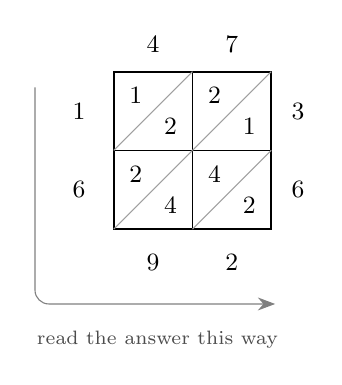
\begin{tikzpicture}[baseline=(current bounding box.north),scale=1.0]
  \lsetup{2}{2}
  \lgrid
  \ltop{1}{4} \ltop{2}{7}
  \lside{1}{3} \lside{2}{6}
  \lcell{1}{1}{1}{2} \lcell{2}{1}{2}{1}
  \lcell{1}{2}{2}{4} \lcell{2}{2}{4}{2}
  \lleft{1}{1} \lleft{2}{6}
  \lbot{1}{9} \lbot{2}{2}
  \lreadarrow
  \node[font=\scriptsize,gray!60!black,anchor=west] at (-1.1,-1.4)
    {read the answer this way};
\end{tikzpicture}
\end{minipage}%
\begin{minipage}[t]{0.56\linewidth}
\vspace{2pt}
$4\times3=12$, \; $7\times3=21$, \; $4\times6=24$, \; $7\times6=42$

\smallskip
Adding the diagonals, starting from the bottom right corner:
\vspace{-2pt}
\begin{align*}
  \text{1st diagonal:}\quad & 2 && = 2\\[-3pt]
  \text{2nd diagonal:}\quad & 4+4+1 && = 9\\[-3pt]
  \text{3rd diagonal:}\quad & 2+2+2 && = 6\\[-3pt]
  \text{4th diagonal:}\quad & 1 && = 1
\end{align*}
\vspace{-14pt}

So $47\times36=1692$.
\end{minipage}
\end{wex}

\begin{enumerate}

\item Both grids below are already filled in. Add along the diagonals and
write the answer. One diagonal in part (b) adds up to more than ten, so you
will need to carry.
\vspace{2pt}

\begin{minipage}[t]{0.5\linewidth}
\centering
(a) $52\times34$\\[4pt]
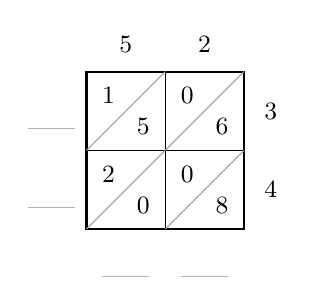
\begin{tikzpicture}[baseline=(current bounding box.north),scale=1.0]
  \lsetup{2}{2}
  \lgrid
  \ltop{1}{5} \ltop{2}{2}
  \lside{1}{3} \lside{2}{4}
  \lcell{1}{1}{1}{5} \lcell{2}{1}{0}{6}
  \lcell{1}{2}{2}{0} \lcell{2}{2}{0}{8}
  \lanslines
\end{tikzpicture}\\[8pt]
$52\times34=\ansline[2cm]$
\end{minipage}%
\begin{minipage}[t]{0.5\linewidth}
\centering
(b) $68\times47$\\[4pt]
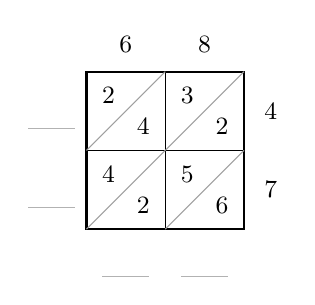
\begin{tikzpicture}[baseline=(current bounding box.north),scale=1.0]
  \lsetup{2}{2}
  \lgrid
  \ltop{1}{6} \ltop{2}{8}
  \lside{1}{4} \lside{2}{7}
  \lcell{1}{1}{2}{4} \lcell{2}{1}{3}{2}
  \lcell{1}{2}{4}{2} \lcell{2}{2}{5}{6}
  \lanslines
\end{tikzpicture}\\[8pt]
$68\times47=\ansline[2cm]$
\end{minipage}

\newpage

\item These grids are drawn but empty. Fill in every cell, then add along the
diagonals. Part (b) has a three-digit number, so its grid has three columns.
\vspace{2pt}

\begin{minipage}[t]{0.42\linewidth}
\centering
(a) $34\times25$\\[4pt]
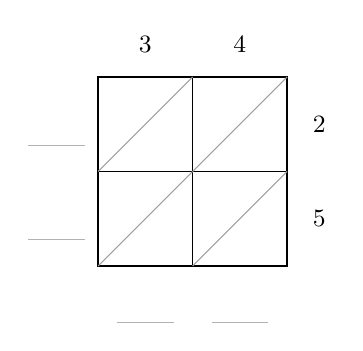
\begin{tikzpicture}[baseline=(current bounding box.north),scale=1.2]
  \lsetup{2}{2}
  \lgrid
  \ltop{1}{3} \ltop{2}{4}
  \lside{1}{2} \lside{2}{5}
  \lanslines
\end{tikzpicture}\\[8pt]
$34\times25=\ansline[2cm]$
\end{minipage}%
\begin{minipage}[t]{0.58\linewidth}
\centering
(b) $243\times17$\\[4pt]
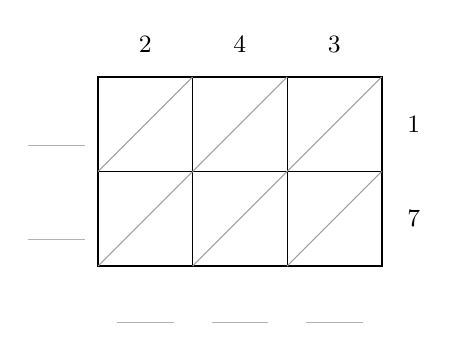
\begin{tikzpicture}[baseline=(current bounding box.north),scale=1.2]
  \lsetup{3}{2}
  \lgrid
  \ltop{1}{2} \ltop{2}{4} \ltop{3}{3}
  \lside{1}{1} \lside{2}{7}
  \lanslines
\end{tikzpicture}\\[8pt]
$243\times17=\ansline[2cm]$
\end{minipage}

\end{enumerate}

\parttitle{2}{Where the decimal point goes}

The lattice method can also be used to multiply decimal numbers. The decimal point in the answer is located on the diagonal where the two decimal points in the numbers being multiplied meet, as seen below.

\begin{wex}{$2.6\times3.4$}
\small
\begin{minipage}[t]{0.40\linewidth}
\centering
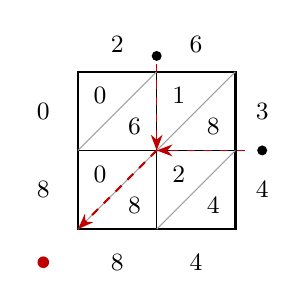
\begin{tikzpicture}[baseline=(current bounding box.north),scale=1.0]
  \lsetup{2}{2}
  \lgrid
  \ltop{1}{2} \ltop{2}{6} \ltopdot{1}
  \lside{1}{3} \lside{2}{4} \lsidedot{1}
  \lcell{1}{1}{0}{6} \lcell{2}{1}{1}{8}
  \lcell{1}{2}{0}{8} \lcell{2}{2}{2}{4}
  \lleft{1}{0} \lleft{2}{8}
  \lbot{1}{8} \lbot{2}{4}
  \ltrace{1}{1}
\end{tikzpicture}
\end{minipage}%
\begin{minipage}[t]{0.60\linewidth}
\vspace{2pt}
The digits along the top are $2$ and $6$, with the decimal point after the
first of them. The digits down the side are $3$ and $4$, again with the decimal
point after the first of them.

\smallskip
Adding the diagonals from the bottom right corner gives $4$, then
$2+8+8=18$, so we write $8$ and carry $1$, then $0+1+6+1=8$, then $0$.

\smallskip
The two dashed lines meet in the middle of the grid, and the diagonal from
there leaves the grid at the bottom left corner. So the digits $0884$ become
$08.84$, which we write as $8.84$.
\end{minipage}
\end{wex}

\begin{enumerate}[resume]

\newpage

\item This grid is already filled in. Add along the diagonals, then use the
decimal points marked on the grid to work out where the decimal point goes in
the answer.
\vspace{2pt}

\begin{center}
\begin{minipage}[t]{0.44\linewidth}
\centering
$1.7\times4.3$\\[4pt]
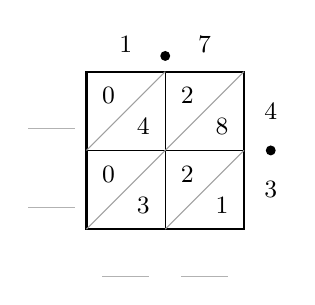
\begin{tikzpicture}[baseline=(current bounding box.north),scale=1.0]
  \lsetup{2}{2}
  \lgrid
  \ltop{1}{1} \ltop{2}{7} \ltopdot{1}
  \lside{1}{4} \lside{2}{3} \lsidedot{1}
  \lcell{1}{1}{0}{4} \lcell{2}{1}{2}{8}
  \lcell{1}{2}{0}{3} \lcell{2}{2}{2}{1}
  \lanslines
\end{tikzpicture}\\[8pt]
$1.7\times4.3=\ansline[2cm]$
\end{minipage}
\end{center}

\item Fill in these grids, then find where the decimal point goes. In part (b)
the decimal points are not in the same place in the two numbers, so the two
lines will not meet in the middle of the grid.
\vspace{2pt}

\begin{minipage}[t]{0.42\linewidth}
\centering
(a) $0.6\times4.5$\\[4pt]
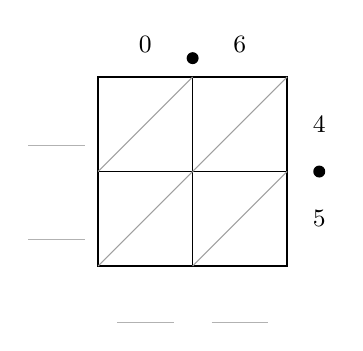
\begin{tikzpicture}[baseline=(current bounding box.north),scale=1.2]
  \lsetup{2}{2}
  \lgrid
  \ltop{1}{0} \ltop{2}{6} \ltopdot{1}
  \lside{1}{4} \lside{2}{5} \lsidedot{1}
  \lanslines
\end{tikzpicture}\\[8pt]
$0.6\times4.5=\ansline[2cm]$
\end{minipage}%
\begin{minipage}[t]{0.58\linewidth}
\centering
(b) $12.4\times0.3$\\[4pt]
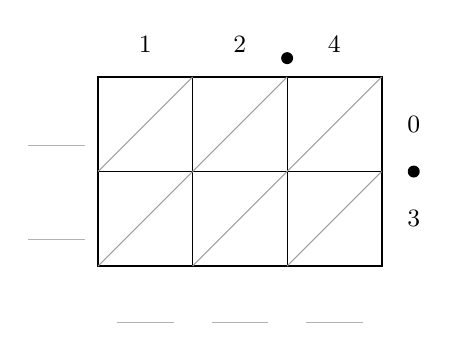
\begin{tikzpicture}[baseline=(current bounding box.north),scale=1.2]
  \lsetup{3}{2}
  \lgrid
  \ltop{1}{1} \ltop{2}{2} \ltop{3}{4} \ltopdot{2}
  \lside{1}{0} \lside{2}{3} \lsidedot{1}
  \lanslines
\end{tikzpicture}\\[8pt]
$12.4\times0.3=\ansline[2cm]$
\end{minipage}

\item Use your answer to Q4 part (a) to write down each of these without
drawing a grid. Explain how you decided where to put the decimal point each
time.
\begin{multicols}{3}
\begin{enumerate}
  \item $6\times45=\ansline[1.5cm]$
  \item $0.06\times4.5=\ansline[1.5cm]$
  \item $60\times0.45=\ansline[1.5cm]$
\end{enumerate}
\end{multicols}
\vspace{13em}

\end{enumerate}

\newpage

\parttitle{3}{Using the method}

The decimal point of a whole number is at the end of its digits, so its mark
goes on the corner of the grid. Everything else about the method stays the
same.

\begin{enumerate}[resume]

\item
\begin{enumerate}
  \item A school orders $24$ packs of pencils. Each pack costs \pounds3.65.
        Use the grid to work out the total cost of the order.
        \vspace{2pt}

        \begin{center}
        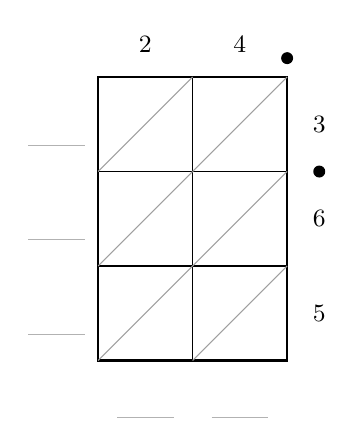
\begin{tikzpicture}[baseline=(current bounding box.north),scale=1.2]
          \lsetup{2}{3}
          \lgrid
          \ltop{1}{2} \ltop{2}{4} \ltopdot{2}
          \lside{1}{3} \lside{2}{6} \lside{3}{5} \lsidedot{1}
          \lanslines
        \end{tikzpicture}
        \end{center}
        \vspace{2pt}
        Total cost: \pounds\ansline[2.5cm]

  \item A dripping tap loses $0.35$ litres of water every hour. Use the grid
        to work out how much water it loses in $16$ hours.
        \vspace{2pt}

        \begin{center}
        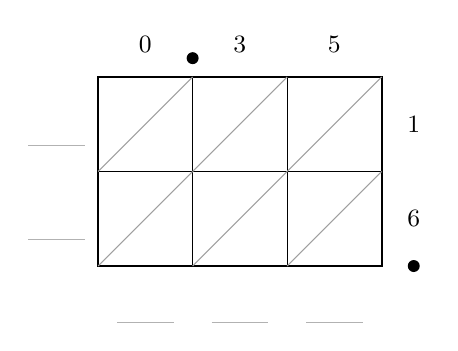
\begin{tikzpicture}[baseline=(current bounding box.north),scale=1.2]
          \lsetup{3}{2}
          \lgrid
          \ltop{1}{0} \ltop{2}{3} \ltop{3}{5} \ltopdot{1}
          \lside{1}{1} \lside{2}{6} \lsidedot{2}
          \lanslines
        \end{tikzpicture}
        \end{center}
        \vspace{2pt}
        Water lost: \ansline[2.5cm] litres
\end{enumerate}

\newpage

\item Draw your own grid for each of these. Mark the decimal points on the
edges of the grid, and show the diagonal you followed to place the decimal
point in the answer.
\vspace{2pt}

\begin{minipage}[t]{0.46\linewidth}
(a) Petrol costs \pounds1.45 per litre. Kofi buys $38$ litres. How much does
he pay?

\vspace{13em}
\end{minipage}\hfill
\begin{minipage}[t]{0.46\linewidth}
(b) A rectangular tile measures $4.8$ cm by $2.5$ cm. What is its area?

\vspace{13em}
\end{minipage}

\item \textbf{Practice.} Use the Chinese multiplication method for each of
these, drawing the grids yourself.
\begin{multicols}{3}
\begin{enumerate}
  \item $73\times48$
  \item $5.2\times3.6$
  \item $0.9\times0.7$
  \item $126\times34$
  \item $8.4\times0.25$
  \item $1.06\times3.5$
\end{enumerate}
\end{multicols}
\vspace{26em}

\end{enumerate}

\newpage

\parttitle{4}{Challenges}

\begin{enumerate}[resume]

\item \textbf{Why the diagonals work.} In the grid for $47\times36$, the cell
holding $4\times6$ and the cell holding $7\times3$ lie on the same diagonal.
\begin{enumerate}
  \item Work out $40\times6$ and $7\times30$. What do you notice about the two
        answers?

        \vspace{6.5em}
  \item Use part (a) to explain why the two cells on that diagonal are added
        together.

        \vspace{7.5em}
\end{enumerate}

\item Sam uses the method on $0.48\times0.25$. His digits come out as
$001200$, and he writes the answer $1200$.
\begin{enumerate}
  \item Without working the multiplication out, explain how you know that
        $1200$ cannot be right.

        \vspace{5.5em}
  \item Draw the grid, place the decimal point, and write down the correct
        answer.

        \vspace{14em}
\end{enumerate}

\newpage

\item How many single-digit multiplications does the method need to work out a
three-digit number multiplied by a four-digit number? Explain how you know
without drawing the grid.

\vspace{9em}

\item Design a multiplication of two numbers, each written to one decimal
place, whose answer is exactly $0.36$. Show that your multiplication works
using the Chinese multiplication method.

\vspace{18em}

\item Zainab says: ``The Chinese multiplication method is better than the
column method, because you never have to carry.'' Use one of your answers from
this sheet to decide whether she is right.

\vspace{13em}

\end{enumerate}

\newpage

\heading{Answers}

{\small
\begin{multicols}{2}
\raggedcolumns
\setlength{\parskip}{4pt}

\textbf{Q1.} (a) The diagonals give $8$, then $0+0+6=6$, then $2+0+5=7$, then
$1$, so $52\times34=1768$. \quad
(b) The diagonals give $6$, then $5+2+2=9$, then $4+3+4=11$, so write $1$ and
carry $1$, then $2+1=3$, so $68\times47=3196$.

\textbf{Q2.} (a) The cells hold $06$, $08$, $15$ and $20$. The diagonals give
$0$, then $2+5+8=15$, so write $5$ and carry $1$, then $1+0+6+1=8$, then $0$,
so $34\times25=850$. \quad
(b) The cells hold $02$, $04$ and $03$ along the top row, and $14$, $28$ and
$21$ along the bottom row. The diagonals give $1$, then $2+8+3=13$, then
$2+4+4+0+1=11$, then $1+0+2+1=4$, then $0$, so $243\times17=4131$.

\textbf{Q3.} The digits are $0731$. Both decimal points sit after the first
digit of their number, so the two lines meet in the middle of the grid and the
diagonal leaves the grid at the bottom left corner: $07.31$, which is $7.31$.

\textbf{Q4.} (a) The cells hold $00$, $24$, $00$ and $30$. The digits are
$0270$ and the diagonal leaves the grid at the bottom left corner, giving
$02.70$, so $0.6\times4.5=2.7$. \quad
(b) The cells hold $00$, $00$ and $00$ along the top row, and $03$, $06$ and
$12$ along the bottom row. The digits are $00372$. The line down from the top
meets the line in from the side one column further to the right, so the
diagonal leaves the grid through the bottom edge, between the third and fourth
digits: $003.72$, so $12.4\times0.3=3.72$.

\textbf{Q5.} (a) $270$ \quad (b) $0.27$ \quad (c) $27$. The digits of the
answer are $27$ every time, because the digits being multiplied have not
changed. Only the place value changes: in (a) both numbers have been multiplied
by $10$, so the answer is $100$ times larger than $2.7$; in (b) the first
number has been divided by $10$, so the answer is $10$ times smaller; in (c)
the first number has been multiplied by $100$ and the second divided by $10$,
so the answer is $10$ times larger.

\textbf{Q6.} (a) The digits are $08760$. The decimal point of $24$ is on the
right-hand corner of the grid, and the diagonal from where the two lines meet
leaves the grid at the bottom left corner, giving $087.60$. The order costs
\pounds$87.60$. \quad
(b) The digits are $00560$, and the decimal point goes between the third and
fourth of them, giving $005.60$. The tap loses $5.6$ litres.

\textbf{Q7.} (a) $1.45\times38=55.10$, so Kofi pays \pounds$55.10$. \quad
(b) $4.8\times2.5=12.00$, so the area is $12$ cm$^2$. The two zeros after the
decimal point do not change the value, so they are not written.

\textbf{Q8.} (a) $3504$ \quad (b) $18.72$ \quad (c) $0.63$ \quad (d) $4284$
\quad (e) $2.1$ \quad (f) $3.71$

\textbf{Q9.} (a) $40\times6=240$ and $7\times30=210$. Both answers are a whole
number of tens, so the digit each one contributes lands in the tens column of
the answer. \quad
(b) A cell does not really hold $4\times6$; it holds $40\times6$, because the
$4$ is in the tens column. Every cell on the same diagonal stands for the same
place value in the answer, which is why the digits on one diagonal are added
together, and why a diagonal totalling ten or more carries into the next
diagonal.

\textbf{Q10.} (a) $0.48$ is less than $1$ and $0.25$ is less than $1$, so the
answer must be smaller than either of them, and certainly smaller than $1$.
Sam's answer is more than a thousand. \quad
(b) The digits are $001200$. The decimal point of $0.48$ is after its first
column and the decimal point of $0.25$ is after its first row, so the two lines
meet one cell in from the top left corner. The diagonal from there leaves the
grid through the left-hand side, between the second and third digits, giving
$00.1200$. So $0.48\times0.25=0.12$.

\textbf{Q11.} $12$ multiplications. The grid has one column for each of the
three digits and one row for each of the four digits, so it has $3\times4=12$
cells, and each cell holds one single-digit multiplication.

\textbf{Q12.} Many answers. For example $0.4\times0.9$, $0.6\times0.6$,
$1.2\times0.3$ and $1.8\times0.2$ all give $0.36$. The digits of the two
numbers have to multiply to $36$, and each number has one digit after the
decimal point, so the answer has two.

\textbf{Q13.} She is partly right. No carrying happens while the grid is being
filled in, because every cell holds a single-digit multiplication and its two
digits have a triangle each. Carrying does still happen when the diagonals are
added: in Q1 part (b) the third diagonal came to $11$, so the $1$ had to be
carried into the next diagonal.

\end{multicols}
}

\end{document}
